
\chapter{Introduction and Objectives}

\label{Intro} 

%%% Introduction and Objectives: This chapter should set the scene for the reader. It must outline the background to the problem, give your reasons for the choice of project, and identify the project’s beneficiaries. Your objectives need to be precisely stated, together with the tests that will show, at the end of the project, that they have been met (or not been met). You need also to outline your methods in broad terms, along with y work plan with sufficient detail to show how you planned to meet the objectives. Outline any major changes of goals or methods that happened during the project. Finally, outline the structure of the report, showing how it fits together.

%-----------------------------------
%	BACKGROUND
%-----------------------------------

\section{Background}

Chammas - 503 words, 7 references
% references
% 1. Self driving robot with Mainframe processor
% 2. European investment, Dickmans
% 3. Carnegie Melon
% 4. Darpa
% 5. Dave
% 6. NVIDIA

% Paragraph 1
% The goal of self driving cars...
% Self-driving cars are a difficult problem to solve...

% Paragraph 2
% With advances in deep learning, training algorithms and computational power...
%% Research question
%% Given the above, how reliable are self-driving cars relying on end-to-end ConvNets in the rain?
%% This project builds on something or other, uses natural and synthetic datasets

%% Practical goal
 The ultimate goal of self-driving cars is to transport people from one place to another without any help from a driver (\cite{s20092544}).
 %% Public health perspective
 From a public health perspective, the overarching
goal of autonomous vehicles is to
transform the current approach
to automotive safety from reducing injuries after collisions to
 complete collision prevention (\cite{Fleetwood_2017}).
%% Business models
Autonomous vehicles fleets allow for new shared autonomous mobility business models 
\cite{riggs2019business}
Shared autonomous electric vehicle (SAEVs) fleets (\cite{loeb2019fleet}. Shared Autonomous Vehicles (SAVs) have gained significant public interest as a possible less expensive, safer and more efficient version of today’s transportation networking companies (TNCs) and taxis.

%% Perceived superiority of AV systems
This perceived superiority to human drivers is attributed to high-performance computing that allows AVs to process, learn from and adjust their guidance systems according
to changes in external conditions at much faster rates than the typical human driver, and it
is supplemented with vehicle-to-vehicle (V2 V) and vehicle-to-infrastructure (V2I) communication, allowing AVs to learn from other vehicles (\cite{west2016moving}).

%% Ethical issues - maybe leave to discussion and further work
safety, liability, privacy, cybersecurity, and industry risks \cite{Taeihagh_2018}

%% Sensor fusion approach
From an interaction, of the vehicle with the travelled path, perspective there are two approaches: the multi-sensor pipeline (Fig. \ref{fig:grigorescu-pipeline} as described by \cite{Grigorescu_2020} and \cite{Yurtsever_2020}. This is the current norm, as can be seen in various 
approach as implemented by (TODO CITATION MISSING), 

\begin{figure}[ht]
 \centering 
 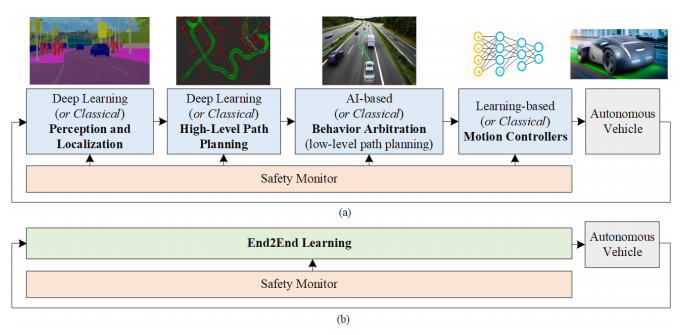
\includegraphics[scale=0.85]{Figures/grigorescu-pipeline.png}
 \caption{Diagrams showing the multisensor pipelline approach (a) and the end to end approach (b) as described by \cite{Grigorescu_2020}}
 \label{fig:grigorescu-pipeline}
\end{figure}



%% End to end approach
and the end to end learning approach as implemented by \cite{bojarski2016end}, training a CNN to map raw pixels from a single front-facing camera directly to steering commands.
\begin{figure}[ht]
 \centering 
 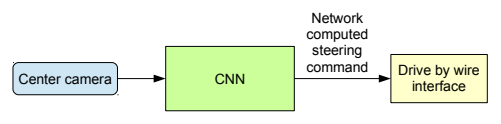
\includegraphics[scale=1]{Figures/bojarski-nvidia.png}
 \caption{Diagram of a trained network with a single centre camera input and a steering command output}
 \label{fig:bojarski-net}
\end{figure}


%% One pixel attacks

\begin{figure}[ht]
 \centering 
 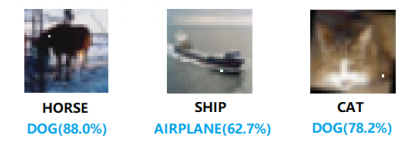
\includegraphics[scale=1]{Figures/one-pixel-attack.png}
 \caption{One-pixel  attacks  created  with the algorithm proposed by \cite{Su_2019} that  successfully  fooled  three  types  of deep neural networks trained  on  CIFAR-10 (\cite{CIFAR_10}) dataset. The modified pixel is white, the original  class  labels  are   black while  the  target  class  labels  and  the corresponding confidence are blue}
 \label{fig:one-pixel-attack}
\end{figure}

Although CNNs have been use successfully for problems in applied to Computer Vision, the robustness of such architectures has been increasingly scrutinised. \cite{Su_2019} proposed an algorithm where a deep neural network, when presented with a images (in this case images from the \cite{CIFAR_10} dataset) with a single pixel change, the network output predicts an incorrect label with a high confidence (Fig. \ref{fig:one-pixel-attack}.  
\cite{zhang2017understanding} demonstrated how traditional benchmarking approaches fail to explain why large neural networks generalize well in practice. By randomizing target labels, the experiments show that state-of-the-art convolutional neural networks for image classification trained with SGD (stochastic gradient descent) are large enough to fit a random labelling of the training data. This is achieved with a simple two-layer neural network, which presents a perfect finite sample expressivity as soon as the number of parameters exceeds the number of data points as usually is the case in practice.

%-----------------------------------
%	AIMS AND OBJECTIVES
%-----------------------------------
\section{Aims and Objectives}

% Chammas - 165 words, no references

The main aim of this project is to determine through a series of experiments how reliable are self driving cars using end to end convolutional neural network architectures, relying solely on raw pixel inputs to predict steering, in the rain, that is, where rainy images are presented to the network. Since the rain pattern is random and can be seen as noise, the expectation is potential for such networks to be fooled and present lower accuracies.

%-----------------------------------
%	BENEFICIARIES
%-----------------------------------
\subsection{Beneficiaries}

Chammas - 79 words, no references

Autonomous vehicles and robotics increasingly rely on computer vision and in some cases convolutional neural networks. The issue of reliability in computer vision based systems when faced with noisy data, in the case of this study, images containing rain, is one that affects every such system using convolutional neural networks, not just autonomous vehicles, hence, any findings in this work could help practitioners to inform designs decisions, industry approval bodies surveying benchmarking methodologies, as well as providing a further advanced starting point for any further research in the area.

%-----------------------------------
%	Introduction to Methods and Work Plan
%-----------------------------------

\section{Introduction to Methods and Work Plan}

Chammas - 130 words, no references

Morbi rutrum odio eget arcu adipiscing sodales. Aenean et purus a est pulvinar pellentesque. Cras in elit neque, quis varius elit. Phasellus fringilla, nibh eu tempus venenatis, dolor elit posuere quam, quis adipiscing urna leo nec orci. Sed nec nulla auctor odio aliquet consequat. Ut nec nulla in ante ullamcorper aliquam at sed dolor. Phasellus fermentum magna in augue gravida cursus. Cras sed pretium lorem. Pellentesque eget ornare odio. Proin accumsan, massa viverra cursus pharetra, ipsum nisi lobortis velit, a malesuada dolor lorem eu neque.

%-----------------------------------
%	Changes in Methods and Work Plan
%-----------------------------------

\subsection{Changes in Methods and Work Plan}

Chammas - 104 words, 1 reference, one image with revised work plan
Morbi rutrum odio eget arcu adipiscing sodales. Aenean et purus a est pulvinar pellentesque. Cras in elit neque, quis varius elit. Phasellus fringilla, nibh eu tempus venenatis, dolor elit posuere quam, quis adipiscing urna leo nec orci. Sed nec nulla auctor odio aliquet consequat. Ut nec nulla in ante ullamcorper aliquam at sed dolor. Phasellus fermentum magna in augue gravida cursus. Cras sed pretium lorem. Pellentesque eget ornare odio. Proin accumsan, massa viverra cursus pharetra, ipsum nisi lobortis velit, a malesuada dolor lorem eu neque.

%-----------------------------------
%	Structure of the report
%-----------------------------------

\section{Structure of the Report}

% Chammas - 324 words, no references
The remaining report is structured as follows:
\begin{itemize}
    \item[--] Chapter 2 provides the critical context, project motivation, methods used, literature survey and analysis. It outlines the current state of research with autonomous vehicles deep neural networks, including ConvNets.
    \item[--] Chapter 3 describes in detail the data and neural network architectures used
    \item[--] Chapter 4 describes the results obtained
    \item[--] Chapter 5 provides a discussion
    \item[--] Chapter 6 provides an evaluation
    \item[--] Appendix A contains the RPMI 363 project proposal
    \item[--] Appendix C contains
    \item[--] Appendix D contains
    \item[--] Appendix E contains
    \item[--] Appendix F contains
    \item[--] Appendix G contains
    \item[--] Additional files have been submitted in the project submission area. These include python source code, unity source code, latex source code, images, URL of online repositories and URLs for data sources used.
\end{itemize}
Sed ullamcorper quam eu nisl interdum at interdum enim egestas. Aliquam placerat justo sed lectus lobortis ut porta nisl porttitor. Vestibulum mi dolor, lacinia molestie gravida at, tempus vitae ligula. Donec eget quam sapien, in viverra eros. Donec pellentesque justo a massa fringilla non vestibulum metus vestibulum. Vestibulum in orci quis felis tempor lacinia. Vivamus ornare ultrices facilisis. Ut hendrerit volutpat vulputate. Morbi condimentum venenatis augue, id porta ipsum vulputate in. Curabitur luctus tempus justo. Vestibulum risus lectus, adipiscing nec condimentum quis, condimentum nec nisl. Aliquam dictum sagittis velit sed iaculis. Morbi tristique augue sit amet nulla pulvinar id facilisis ligula mollis. Nam elit libero, tincidunt ut aliquam at, molestie in quam. Aenean rhoncus vehicula hendrerit.